\section{MOS-Diode\skript{Kap. 7}}
Für Kennlinien der MOS-Dioden siehe Abbildung \ref{fig:diodenKennlinien}.
\begin{figure}[h]
	\centering
	\begin{subfigure}[b]{5cm}
		\centering
		{\begin{circuitikz}[european voltages]
	\draw (0,0) to[full diode, i=$I_D$] (0,-2);
	\draw[->, thick] (-0.7,-0.2) -- (-0.7,-1.8) node[midway, left] {$V_D$};
\end{circuitikz}}
		\caption{Ideale Diode ($V_F = V_{F0}$)}
	\end{subfigure}
	\begin{subfigure}[b]{4cm}
		\centering
		{\begin{circuitikz}[european voltages]
	\draw (0,0) to[full diode, i=$I_D$] (0,-2);
	\draw[->, thick] (-0.7,-0.2) -- (-0.7,-1.8) node[midway, left] {$V_D$};
\end{circuitikz}}
		\caption{Reale Diode}
	\end{subfigure} \quad
	\begin{subfigure}[b]{4cm}
		\centering
		{\begin{circuitikz}[european voltages]
	\ctikzset{tripoles/mos style/arrows}
	\draw (0,-1) to[Tnmos, n=n1] (0,0);
	\draw (n1.source) to[short, i=$I_D$] (0,-2);
	\draw (n1.gate) |- (n1.drain) -- +(0,0.5);
	\draw[->, thick] (-1.2,0.5) -- (-1.2,-1.5) node[midway, left] {$V_{GS}$};
\end{circuitikz}}
		\caption{n-Kanal}
	\end{subfigure}
	\begin{subfigure}[b]{4cm}
		\centering
		{\begin{circuitikz}[european voltages]
	\ctikzset{tripoles/mos style/arrows}
	\draw (0,-1) to[Tpmos, n=n1] (0,0);
	\draw (n1.source) to[short, i<=$I_D$] +(0,0.4);
	\draw (n1.gate) |- (n1.drain) -- +(0,-0.5);
	\draw[->, thick] (0.5,0) -- +(0,-1.5) node[midway, right] {$V_{GS}$};
\end{circuitikz}}
		\caption{p-Kanal}
	\end{subfigure}
	\hspace{1.5cm}
	
	\begin{subfigure}[b]{4cm}
		{\begin{tikzpicture}
	\draw[->] (0,0) -- (0,3.5) node[left] {$I_D$};
	\draw[->] (0,0) -- (3.5,0) node[below] {$V_D$};
	\draw (0, 0.04) -- ++(2,0) -- +(0,3);
\end{tikzpicture}}
	\end{subfigure} \quad
	\begin{subfigure}[b]{4cm}
		\centering
		{\begin{tikzpicture}
	\draw[->] (0,0) -- (0,3.5) node[left] {$I_D$};
	\draw[->] (0,0) -- (3.5,0) node[below] {$V_D$};
	\draw (0, 0.04) -- ++(1.2,0);
	\draw (1.2,0.04) .. controls (1.5,0.04) and (1.7,2.8) .. (1.7,2.8);
	\draw (2,3.3) node {$I_D = I_S (e^{\frac{V_D}{\Phi_t}}  -1)$};
\end{tikzpicture}}
	\end{subfigure} \qquad
	\begin{subfigure}[b]{8cm}
		\centering
		{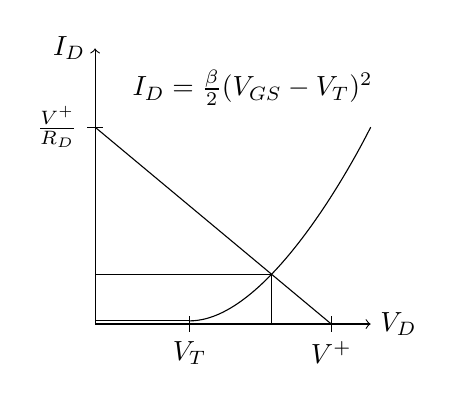
\begin{tikzpicture}
	\draw[->] (0,0) -- (0,3.5) node[left] {$I_D$};
	\draw[->] (0,0) -- (3.5,0) node[right] {$V_D$};
	\draw (0, 0.04) -- ++(1.2,0);
	\draw (1.2,0.04) .. controls (2.3,0.04) and (3.5,2.5) .. (3.5,2.5);
	\draw (2,3) node {$I_D = \frac{\beta}{2}(V_{GS} -V_T)^2$};
	\draw (1.2,0.1) -- +(0,-0.2) node[below] {$V_T$};
	\draw (0,0.63) -- ++(2.242,0) --  +(0,-0.63);
	\draw (0,2.5) -- (3,0);
	\draw (-0.1, 2.5) -- +(0.2,0);
	\draw (-0.1, 2.5) node[left] {$\frac{V^+}{R_D}$};
	\draw (3, 0.1) -- +(0, -0.2) node[below] {$V^+$};
\end{tikzpicture}}
	\end{subfigure}			
	\caption{Gegenüberstellung Dioden-Kennlinien}
	\label{fig:diodenKennlinien}
\end{figure}

\begin{figure}[h]
	\centering
	\begin{subfigure}[b]{5cm}
		\centering
		{\begin{circuitikz}[american, european resistors]
	\draw (0,0) node[circ, name=G] {} node[left] {G};
	\draw (4,0) node[circ, name=D] {} node[right] {D};
	\draw (4,-2) node[circ, name=S] {} node[right] {S};
	\draw (0,-2) -- (S);
	\draw (G) -- +(3,0);
	\draw (3,0) to[R=$\frac{1}{g_0}$] +(0,-2);
	\draw (2,0) to[I_=$g_m v_{GS}$] +(0,-2);
	\draw (D) to[short, i_=$i_D$] +(-1,0);
	\draw[->, thick] (0, -0.2) -- +(0,-1.6) node[midway, left] {$v_{GS}$};
\end{circuitikz}}
	\end{subfigure} \qquad\qquad
	\begin{subfigure}[b]{3cm}
		\centering
		{\begin{circuitikz}[american, european resistors]
	\draw (4,0) node[circ, name=D] {} node[right] {D};
	\draw (4,-2) node[circ, name=S] {} node[right] {S};
	\draw (1.5,-2) -- (S);
	\draw (3,0) to[R=$\frac{1}{g_0}$] +(0,-2);
	\draw (3,0) -- (1.5,0) to[R=$\frac{1}{g_m}$] +(0,-2);
	\draw (D) to[short, i_=$i_D$] +(-1,0);
\end{circuitikz}}
	\end{subfigure}
	\caption{Ersatzschaltungen der MOS-Diode}
\end{figure}

\begin{tabular}{|l|l|}
	\hline
	Arbeitspunktstrom einer MOS-Diode mit Wiederstandslast $R_D$
	& $I_D = \frac{\beta}{2} (V_{GS} -V_T)^2 = \frac{V^+ - V_{GS}}{R_D} $
	\\ \hline
	Drain-Source Spannung einer MOS-Diode bei gegebenem Strom
	& $ V_{GS} = V_T + \sqrt{\frac{2I_D}{\beta(1+\lambda V_{DS})}} \approx V_T + \sqrt{\frac{2I_D}{\beta}} $
	\\ \hline
	Innenwiderstand der MOS-Diode
	& $ r_{MD} = \frac{v_{GS}}{i_D} = \frac{1}{g_m + g_0} \approx \frac{1}{g_m} $
	\\ \hline	
\end{tabular}

